\section{Output}
\subsection{Files}

Explain the created C++ files and executables, and how to use them.

\subsection{Two-scale algorithm}

Explain the structure of the two-scale algorithm classes and how they
work and are plugged together.


The stucture of the two-scale algorithm used in \flexisusy\ is as follows,%

Initial guess:
\begin{enumerate}
\item Guess gauge couplings $g_{1,2,3}$ at $m_Z$
\item Apply user-defined low-scale constraint (\code{LowScaleInput})
\item Guess Yukawa couplings $y^{u,d,e}_{ij}$ at $m_Z$
\item Run model to the high-scale (\code{HighScaleFirstGuess})
\item Apply high-scale constraint (\code{HighScaleInput})
\item Run model to the low-scale (\code{LowScaleFirstGuess})
\item Solve EWSB eqs.\ at the tree-level
\item Calculate \DRbar\ masses
\end{enumerate}
%
Solving the renormalization group equations:
\begin{enumerate}
\item \label{rge-step-one} Run model to the low-scale (\code{LowScale})
  \begin{enumerate}
  \item Calculate \DRbar\ masses
  \item Recalculate low-scale
  \item Calculate \DRbar\ gauge and Yukawa couplings $g_{1,2,3}$,
    $y^{u,d,e}_{ij}$, see
    Section~\ref{sec:matching-to-the-standard-model}.
  \item Apply user-defined low-scale constraint (\code{LowScaleInput})
  \end{enumerate}
\item Run model to the high-scale (\code{HighScale})
  \begin{enumerate}
  \item Recalculate high-scale
  \item Apply high-scale constraint (\code{HighScaleInput})
  \end{enumerate}
\item Run model to the susy-scale (\code{SUSYScale})
  \begin{enumerate}
  \item Calculate \DRbar\ masses
  \item Recalculate low-scale
  \item Apply susy-scale constraint (\code{SUSYScaleInput})
  \item Solve EWSB eqs.\ at the one-loop level
  \end{enumerate}
\item If not converged yet, goto \ref{rge-step-one}
\end{enumerate}
%
Calculating the particle spectrum:
\begin{enumerate}
\item Run model to the susy-scale
\item Calculate the pole masses
\item Run model to the parameter output scale (SLHA block MODSEL 12)
\end{enumerate}

\begin{figure}[tb]
  \centering
  \tikzumlset{fill class=white}
  \begin{tikzpicture}
    \umlclass[x=0, y=0, type=abstract]{Beta\_function}{
      -- scale : double\\
      -- loops : unsigned\\
      -- numPars : unsigned
    }{
      + \umlvirt{display() : const Eigen::ArrayXd} \\
      + \umlvirt{set(v : const Eigen::ArrayXd\&) : void}\\
      + \umlvirt{beta() : Eigen::ArrayXd}\\
      + run\_to(scale : double, eps : double) : void\\
    }
    \umlclass[x=8, y=-12, template={T}]{MSSM}{}{}
    \umlclass[x=8, y=-8, type=abstract]{Two\_scale\_model}{}{
      + \umlvirt{calculate\_spectrum() : void}\\
      + \umlvirt{run\_to(scale : double, eps : double) : void}\\
      + \umlvirt{set\_precision(precision : double) : void}
    }
    \umlclass[x=0, y=-4]{MSSM\_susy\_parameters}{}{
      + display() : const Eigen::ArrayXd \\
      + set(v : const Eigen::ArrayXd\&) : void\\
      + beta() : Eigen::ArrayXd
    }
    \umlclass[x=0, y=-8]{MSSM\_soft\_parameters}{}{
      + display() : const Eigen::ArrayXd \\
      + set(v : const Eigen::ArrayXd\&) : void\\
      + beta() : Eigen::ArrayXd
    }
    \umlclass[x=0, y=-12]{MSSM$<$Two\_scale$>$}{}{
      + calculate\_spectrum() : void\\
      + run\_to(scale : double, eps : double) : void\\
      + set\_precision(precision : double) : void
    }
   \umlinherit{MSSM\_susy\_parameters}{Beta\_function}
   \umlinherit{MSSM\_soft\_parameters}{MSSM\_susy\_parameters}
   \umlinherit{MSSM$<$Two\_scale$>$}{MSSM\_soft\_parameters}
   \umlinherit{MSSM$<$Two\_scale$>$}{Two\_scale\_model}
   \umldep[arg1={$<<$bind$>>$}, mult1={T $\rightarrow$ Two\_scale}, pos1=0.5]{MSSM$<$Two\_scale$>$}{MSSM}
  \end{tikzpicture}
  \caption{Two-scale model class hierarchy}
  \label{fig:two-scale-model-class-hierarchy}
\end{figure}

\begin{figure}[tb]
  \centering
  \tikzumlset{fill class=white}
  \begin{tikzpicture}
    \umlclass[x=0, y=0, type=abstract]{Two\_scale\_model}{}{
      + \umlvirt{calculate\_spectrum() : void}\\
      + \umlvirt{run\_to(scale : double, eps : double) : void}\\
      + \umlvirt{set\_precision(precision : double) : void}
    }
    \umlclass[x=0, y=-4]{RGFlow$<$Two\_scale$>$}{}{
      + solve() : void
    }
    \umlclass[x=8, y=0]{Constraint$<$Two\_scale$>$}{}{
      + \umlvirt{apply() : void}\\
      + \umlvirt{get\_scale() : double}\\
      + \umlvirt{set\_model(model : Two\_scale\_model*) : void}
    }
    \umlclass[x=8, y=4, template={T}]{Constraint}{}{}
    \umlclass[x=0, y=-7]{Initial\_guesser$<$Two\_scale$>$}{}{
      + \umlvirt{guess() : void}
    }
    \umlclass[x=0, y=-11, template={T}]{Initial\_guesser}{}{}
    \umlclass[x=8, y=-7]{Convergence\_tester$<$Two\_scale$>$}{}{
      + \umlvirt{accuracy\_goal\_reached() : bool}\\
      + \umlvirt{max\_iterations() : unsigned}
    }
    \umlclass[x=8, y=-11, template={T}]{Convergence\_tester}{}{}
    \umlclass[x=8, y=-4, template={T}]{RGFlow}{}{}
    \umldep[arg1={$<<$bind$>>$}, mult1={T $\rightarrow$ Two\_scale}, pos1=0.5]{RGFlow$<$Two\_scale$>$}{RGFlow}
    \umldep[mult1=1..*]{RGFlow$<$Two\_scale$>$}{Two\_scale\_model}
    \umldep[mult1=1..*]{RGFlow$<$Two\_scale$>$}{Constraint$<$Two\_scale$>$}
    \umldep{RGFlow$<$Two\_scale$>$}{Initial\_guesser$<$Two\_scale$>$}
    \umldep{RGFlow$<$Two\_scale$>$}{Convergence\_tester$<$Two\_scale$>$}
    \umldep[mult1={$<<$bind$>>$}, arg1={T $\rightarrow$ Two\_scale}, pos1=0.5]{Initial\_guesser$<$Two\_scale$>$}{Initial\_guesser}
    \umldep[mult1={$<<$bind$>>$}, arg1={T $\rightarrow$ Two\_scale}, pos1=0.5]{Convergence\_tester$<$Two\_scale$>$}{Convergence\_tester}
    \umldep[arg1={$<<$bind$>>$}, mult1={T $\rightarrow$ Two\_scale}, pos1=0.5]{Constraint$<$Two\_scale$>$}{Constraint}
  \end{tikzpicture}
  \caption{Two-scale renormalization group solver class hierarchy}
  \label{fig:two-scale-rgflow-class-hierarchy}
\end{figure}

\subsubsection{Matching to the Standard Model}
\label{sec:matching-to-the-standard-model}

\paragraph{Gauge couplings}

At the low-scale $M_Z$ we calculate
%
\begin{align}
  \alpha_{\text{e.m.},\text{susy}}^{\text{\DRbar}}(M_Z) &=
  \frac{\alpha_{\text{e.m.},\text{SM}}^{(5),\text{\MSbar}}(M_Z)}{1 -
    \Delta\alpha_{\text{e.m.},\text{SM}}(M_Z) -
    \Delta\alpha_{\text{e.m.},\text{susy}}(M_Z)} ,\\
  \Delta\alpha_{\text{e.m.},\text{SM}}(\mu) &=
  \frac{\alpha_\text{e.m.}}{2\pi} \left[\frac{1}{3}
    - \frac{16}{9} \log{\frac{m_t}{\mu}} \right],\\
  \Delta\alpha_{\text{e.m.},\text{susy}}(\mu) &=
  \frac{\alpha_\text{e.m.}}{2\pi} \left[ -\sum_{\text{susy particle }
      i}
    C_i \log{\frac{m_i}{\mu}} \right],\\
    e_{\text{susy}}^{\text{\DRbar}}(M_Z) &=
    \sqrt{4\pi\alpha_{\text{e.m.},\text{susy}}^{\text{\DRbar}}(M_Z)}
\end{align}
%
\begin{align}
  \alpha_{\text{s},\text{susy}}^{\text{\DRbar}}(M_Z) &=
  \frac{\alpha_{\text{s},\text{SM}}^{(5),\text{\MSbar}}(M_Z)}{1 -
    \Delta\alpha_{\text{s},\text{SM}}(M_Z)
    - \Delta\alpha_{\text{s},\text{susy}}(M_Z)} ,\\
  \Delta\alpha_{\text{s},\text{SM}}(\mu) &=
  \frac{\alpha_\text{s}}{2\pi} \left[
    -\frac{2}{3} \log{\frac{m_t}{\mu}} \right],\\
  \Delta\alpha_{\text{s},\text{susy}}(\mu) &=
  \frac{\alpha_\text{s}}{2\pi}\left[ \frac{1}{2}-\sum_{\text{susy
        particle } i} C_i \log{\frac{m_i}{\mu}} \right] ,\\
  g_{3,\text{susy}}^{\text{\DRbar}}(M_Z) &=
  \sqrt{4\pi\alpha_{\text{s},\text{susy}}^{\text{\DRbar}}(M_Z)} ,
\end{align}
%
where
%
\begin{align}
  \alpha_{\text{e.m.},\text{SM}}^{(5),\text{\MSbar}}(M_Z) &= 1/127.944,\\
  \alpha_{\text{s},\text{SM}}^{(5),\text{\MSbar}}(M_Z) &= 0.1185,
\end{align}
%
are the \MSbar electromagnetic and strong cougling constants in the
Standard Model including only $5$ quark flavours
\cite{Beringer:1900zz}.  Afterwards, SARAH's tree-level expressions
for the Weinberg angle and the Hypercharge and left gauge couplings
$g_Y$ and $g_2$ in terms of $M_{W,\text{susy}}^{\text{\DRbar}}(M_Z)$,
$M_{Z,\text{susy}}^{\text{\DRbar}}(M_Z)$ and
$e_{\text{susy}}^{\text{\DRbar}}(M_Z)$ are used to calculate
$g_{1,\text{susy}}^{\text{\DRbar}}(M_Z)$ and
$g_{2,\text{susy}}^{\text{\DRbar}}(M_Z)$.  In the MSSM, for example,
we'll have
%
\begin{align}
  \theta_{W,\text{susy}}^{\text{\DRbar}}(M_Z) &=
  \arcsin\sqrt{1 - \left(\frac{M_{W,\text{susy}}^{\text{\DRbar}}(M_Z)}{M_{Z,\text{susy}}^{\text{\DRbar}}(M_Z)}\right)^2} ,\\
  g_{1,\text{susy}}^{\text{\DRbar}}(M_Z) &=
  \sqrt{\frac{5}{3}} \frac{e_{\text{susy}}^{\text{\DRbar}}(M_Z)}{\cos\theta_{W,\text{susy}}^{\text{\DRbar}}(M_Z)} ,\\
  g_{2,\text{susy}}^{\text{\DRbar}}(M_Z) &=
  \frac{e_{\text{susy}}^{\text{\DRbar}}(M_Z)}{\sin\theta_{W,\text{susy}}^{\text{\DRbar}}(M_Z)} ,
\end{align}
%
where
%
\begin{align}
  \left(M_{W,\text{susy}}^{\text{\DRbar}}(M_Z)\right)^2 &=
  \left(M_W^{\text{pole}}\right)^2 + \re \Pi_{WW}^T(p^2 = (M_W^{\text{pole}})^2) ,\\
  \left(M_{Z,\text{susy}}^{\text{\DRbar}}(M_Z)\right)^2 &=
  \left(M_Z^{\text{pole}}\right)^2 + \re \Pi_{ZZ}^T(p^2 = (M_Z^{\text{pole}})^2)
\end{align}
%
and $M_W^{\text{pole}} = 80.404\unit{GeV}$, $M_Z^{\text{pole}} =
91.1876\unit{GeV}$ \cite{Beringer:1900zz}.

\paragraph{Fermion masses}

\begin{align}
  \left(y_u^{\text{\DRbar}}(M_Z)\right)_{ij} &= \frac{\sqrt{2} m_{u,ji}}{v_u} ,\\
  \left(y_d^{\text{\DRbar}}(M_Z)\right)_{ij} &= \frac{\sqrt{2} m_{d,ji}}{v_d} ,\\
  \left(y_e^{\text{\DRbar}}(M_Z)\right)_{ij} &= \frac{\sqrt{2} m_{e,ji}}{v_e} ,
\end{align}
%
where the fermion mass matrices are given by
%
\begin{align}
  m_{u,11} &= m_{u}^{\userinput} ,\\
  m_{u,22} &= m_{c}^{\userinput} ,\\
  m_{u,33} &= m_{t,\text{susy}}^{\text{\DRbar}}(M_Z),\\
  m_{d,11} &= m_{d}^{\userinput} ,\\
  m_{d,22} &= m_{s}^{\userinput} ,\\
  m_{d,33} &= m_{b,\text{susy}}^{\text{\DRbar}}(M_Z),\\
  m_{e,11} &= m_{e}^{\userinput} ,\\
  m_{e,22} &= m_{\mu}^{\userinput} ,\\
  m_{e,33} &= m_{\tau,\text{susy}}^{\text{\DRbar}}(M_Z),\\
  m_{u,ij} &= m_{d,ij} = m_{u,ij} = 0 \quad \forall i \neq j.
\end{align}
%
Only the 3rd generation quark masses are calculated in the \DRbar
scheme from the user input quantities $m_t^\text{pole}$,
$m_{b,\text{SM}}^{\text{\MSbar}}(M_Z)$,
$m_{\tau,\text{SM}}^{\text{\MSbar}}(M_Z)$.  The top quark \DRbar mass
is calculated via
%
\begin{align}
  m_{t,\text{susy}}^{\text{\DRbar}}(\mu) &= m_t^\text{pole}
  + \re\Sigma_{tt}^{S,\text{heavy}}(m_t^\text{pole})
  + m_t^\text{pole} \left[
    \re\Sigma_{tt}^{L,\text{heavy}}(m_t^\text{pole}) +
    \re\Sigma_{tt}^{R,\text{heavy}}(m_t^\text{pole}) +
    \Delta m_t^{(1),\text{qcd}} +
    \Delta m_t^{(2),\text{qcd}}
  \right].
\end{align}
%
The QCD contributions $\Delta m_t^{(1),\text{qcd}}$ and $\Delta
m_t^{(2),\text{qcd}}$ are taken from \cite{Bednyakov:2002sf} and read
%
\begin{align}
  \Delta m_t^{(1),\text{qcd}} &= -\frac{g_3^2 \left(5-3 \log\left(\frac{m_t^2}{\mu^2}\right)\right)}{12 \pi^2},\\
  \Delta m_t^{(2),\text{qcd}} &= \left(\Delta
    m_t^{(1),\text{qcd}}\right)^2 - \frac{g_3^4 \left[396
      \log^2\left(\frac{m_t^2}{\mu^2}\right)-1476
      \log\left(\frac{m_t^2}{\mu^2}\right)-48 \zeta(3)+2011+16 \pi ^2
      (1+\log(4))\right]}{4608 \pi^4}.
\end{align}
%
The \DRbar mass of the bottom quark is calculated via
\cite{Baer:2002ek}
%
\begin{align}
  m_{b,\text{susy}}^{\text{\DRbar}}(\mu) &=
  \frac{m_{b,\text{SM}}^{\text{\DRbar}}(\mu)}{1 -
    \re\Sigma_{bb}^{S,\text{heavy}}(m_{b,\text{SM}}^\text{\MSbar})/m_b
    - \re\Sigma_{bb}^{L,\text{heavy}}(m_{b,\text{SM}}^\text{\MSbar}) -
    \re\Sigma_{bb}^{R,\text{heavy}}(m_{b,\text{SM}}^\text{\MSbar})} ,\\
  m_{b,\text{SM}}^{\text{\DRbar}}(\mu) &=
  m_{b,\text{SM}}^{\text{\MSbar}}(\mu) \left(1 - \frac{\alpha_s}{3
      \pi} - \frac{23}{72} \frac{\alpha_s^2}{\pi^2} + \frac{3
      g_2^2}{128 \pi^2} + \frac{13 g_1^2}{1152 \pi^2}\right) .
\end{align}
%
The \DRbar mass of the $\tau$ is calculated via
%
\begin{align}
  m_{\tau,\text{susy}}^{\text{\DRbar}}(\mu) &=
  m_{\tau,\text{SM}}^{\text{\DRbar}}(\mu) +
  \re\Sigma_{\tau\tau}^{S,\text{heavy}}(m_{\tau,\text{SM}}^\text{\MSbar}) +
  m_{\tau,\text{SM}}^{\text{\DRbar}}(\mu) \left[
    \re\Sigma_{\tau\tau}^{L,\text{heavy}}(m_{\tau,\text{SM}}^\text{\MSbar}) +
    \re\Sigma_{\tau\tau}^{R,\text{heavy}}(m_{\tau,\text{SM}}^\text{\MSbar})
  \right] ,\\
  m_{\tau,\text{SM}}^{\text{\DRbar}}(\mu) &= m_{\tau,\text{SM}}^{\text{\MSbar}}(\mu)
  \left(1 - 3 \frac{g_1^2 - g_2^2}{128 \pi^2}\right).
\end{align}

\subsection{Lattice algorithm}

Explain the structure of the lattice algorithm classes and how they
work.
